% ****** Start of file .tex ******
%
%   This file is based on apssamp.tex, part of the APS files in the REVTeX 4.1 distribution.
%   Version 4.1r of REVTeX, August 2010
%
%   Copyright (c) 2009, 2010 The American Physical Society.
%   Samuel Balula, Pedro Ribeiro, Luís Macedo, Eduardo Neto 2013
%   See the REVTeX 4 README file for restrictions and more information.
%
% TeX'ing this file requires that you have AMS-LaTeX 2.0 installed
% as well as the rest of the prerequisites for REVTeX 4.1
%
% See the REVTeX 4 README file
% It also requires running BibTeX. The commands are as follows:
%
%  1)  latex filename.tex
%  2)  bibtex filename
%  3)  latex filename.tex
%  4)  latex filename.tex

\documentclass[%
  reprint,
  %superscriptaddress,
  %groupedaddress,
  %unsortedaddress,
  %runinaddress,
  %frontmatterverbose, 
  %preprint,
  %showpacs,preprintnumbers,
  nofootinbib,
  %nobibnotes,
  %bibnotes,
  amsmath,amssymb,
  aps,
  %pra,
  %prb,
  %rmp,
  %prstab,
  %prstper,
  %floatfix,
  10pt,
  a4paper
]{revtex4-1}



\usepackage{facil}                      % Pacote pessoal
\usepackage{verbatim}                   % Apresentação de código
\usepackage{graphicx}                   % Include figure files
\usepackage{dcolumn}                    % Align table columns on decimal point
\usepackage{bm}                         % bold math
\usepackage[latin1,utf8]{inputenc}      % Tipos de caracteres
\usepackage[portuges]{babel}            % Português
\usepackage{indentfirst}                % Identação da primeira linha
\usepackage{hyperref}                   % add hypertext capabilities
\usepackage{float}                      %Fixar imagens
%\usepackage[mathlines]{lineno}          % Enable numbering of text and display math
%\linenumbers\relax                      % Commence numbering lines
%\usepackage[compact]{titlesec}

\usepackage[%showframe,%Uncomment any one of the following lines to test 
%%scale=0.7, marginratio={1:1, 2:3}, ignoreall, % default settings
%%text={7in,10in},centering,
margin=0.5in,        %diminuir margens
%total={6.5in,8.75in}, top=1.2in, left=0.9in, 
includefoot
%height=10in,a5paper,hmargin={3cm,0.8in},
]{geometry}

\begin{document}
\preprint{APS/123-QED}
%\captionsetup[table]{font=small,skip=0pt}
%\captionsetup[figure]{font=small,skip=0pt}
%\titlespacing{\section}{0pt}{*0}{*0}            %Poupar espaço
%\titlespacing{\subsection}{0pt}{*0}{*0}
%\titlespacing{\subsubsection}{0pt}{*0}{*0}


% % % % % % % % % % % % % % % % % % % % % % % % % % % % % % % % % % % % % % % % 
%%%%%%%%%%%%%%%%%%%%%%%%%%%%%%%%%% Início %%%%%%%%%%%%%%%%%%%%%%%%%%%%%%%%%%%%%%
% % % % % % % % % % % % % % % % % % % % % % % % % % % % % % % % % % % % % % % %
 

\title{Levitação magnética com electroiman e fotoresistência}
%\thanks{}

\author{Pedro Ribeiro}%
\email{73221, pedro.q.ribeiro@tecnico.ulisboa.pt}
\author{Luis Macedo}%
\email{73633, luis.macedo@tecnico.ulisboa.pt}
\author{Samuel Balula}%
\email{72735, samuel.balula@tecnico.ulisboa.pt}

\affiliation{
  Instituto Superior Técnico\\
  Mestrado em Engenharia Física Tecnológica\\
  Complementos de Electrónica
}

%\collaboration{Grupo 57}

\date{\today}

%%%%%%%%%%%%%%%%%%%%%%%%%%%%%%%%%% Abstract %%%%%%%%%%%%%%%%%%%%%%%%%%%%%%%%%%%%
\begin{abstract}
Neste trabalho laboratorial implementa-se um sistema de controlo que mantem em levitação um objeto metálico não magnetizado.
......................................
%1


\end{abstract}
\maketitle


%%%%%%%%%%%%%%%%%%%%%%%%%%%%%%%%%% Introdução %%%%%%%%%%%%%%%%%%%%%%%%%%%%%%%%%%
\section{Introdução}
\label{s:intro}
%Situar o problema, incluir fórmulas.
%Quem lê o relatório deve conseguir perceber exatamente o que foi feito.
%2

%%%%%%%%%%%%%%%%%%%%%%%%%%%% Experiência realizada %%%%%%%%%%%%%%%%%%%%%%%%%%%%%
\section{Experiência Realizada}
\label{s:expreal}
%Incluir diagrama de blocos da montagem
De acordo com as instruções do guia, implentou-se o circuito da \rfig{../img/esquematico.png}. Apresentam-se na tabela \ref{partlist} os componentes eléctricos utilizados, montados numa breadboard.

\figurao{../img/esquematico.png}{Circuito implementado no laboratório}

\tabela[partlist]{Lista dos componentes utilizados}{lrrr}{
	Descrição		&Modelo/Valor		&Qt.			&Referência	\\ \hline
	Bobine c/ núcleo ferro	&			&1			&L1		\\
	Fotoresistência		&			&1			&R3		\\
	Trans. J. Bipolar NPN	&2N3055			&1			&Q1		\\
	Trans. J. Bipolar PNP	&MJ2955			&1			&Q2		\\
	Ampl. operacional	&LM741			&5			&UX		\\
	LED			&red			&1			&LED		\\
	Cond. electrolítico	&1$\mu$F		&1			&C1		\\
	Potenciómetro		&10K$\Omega$		&1			&R5		\\
	Resistência .25W	&100$\Omega$		&1			&R0		\\
	Resistência .25W	&300$\Omega$		&1			&R4		\\
	Resistência .25W	&1K$\Omega$		&1			&R10		\\
	Resistência .25W	&2.2K$\Omega$		&1			&R12		\\
	Resistência .25W	&5.6K$\Omega$		&1			&R1		\\
	Resistência .25W	&10K$\Omega$		&1			&R2		\\
	Resistência .25W	&15K$\Omega$		&1			&R11		\\
	Resistência .25W	&56K$\Omega$		&4			&R6-9		\\
	%3
}

Para facilidade de análise, divide-se o circuito nas suas partes constituintes, que se analisam separadamente.


\subsection{LED}
%4
\fig[.2]{../img/led.png}{Circuito do LED}

Para iluminar um led, colocado em frente à fotoresistência, utilizou-se o circuito da \rfig{../img/led.png}. Para a tensão de alimentação de cerca de 10V utilizada, a corrente é dada por \eqref{eled}. O valor é suficientemente alto para que a intensidade da radiação emitida influence a resistência variável fotosensível, estando dentro dos limites eléctricos de funcionamento.

\eq[eled]{I=\frac{V_{cc}-V_d}{R_0} \approx 93 mA}
	
	
\subsection{Divisor de Tensão}
%Da a tensao de referencia
%5

\fig{../img/divtensao.png}{Excerto do esquemático representando o divisor de tensão}

O circuito apresentado na \rfig{../img/divtensao.png} é um simples divisor de tensão, formado pelas resistências R1 e R2, e um seguidor de tensão, em que se usa um amplificador operacional LM741. Para uma tensão de referência de 10V, obtÊm-se uma referência de 3.6V. Utiliza-se este divisor afim de evitar tensões (e correntes) excessivas nos andares seguintes, em particular tendo em conta a fotoresistência, que pode apresentar resistências da ordem das centenas de $\Omega$.






\subsection{Fotoresistência}
%6
Uma fotoresistência é um componente composto por um material que sofre variação da sua resistividade com a variação da intensidade da luz incidente neste (também conhecido como fotocondutividade).\\
O dispositivo utilizado sofria um aumento da sua condutividade (e consequentemente uma diminuição da resistência) com o aumento da intensidade luminosa. Integrando este dispositivo num divisor de tensão, como se mostra na figura \ref{fig:foto_res}, que obedece à relação:
\begin{equation}
V_{out}=\frac{R_3}{R_3+R_4}V_{in}
\label{eq:div_t}
\end{equation}
\begin{figure}
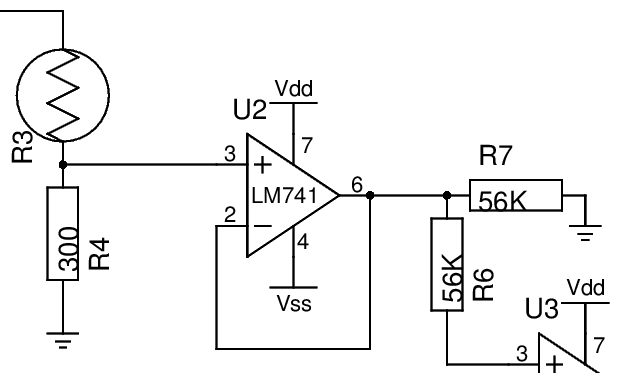
\includegraphics[width=3in]{../img/sensor.png}
\caption{Esquemático do divisor de tensão de tensão onde se inseriu o sensor ($R_3$) com seguidor de tensão.}
\label{fig:foto_res}
\end{figure}
Desta forma, e de acordo com a relação obtida em \ref{eq:div_t}, o sinal de saída do divisor de tensão será tanto maior quanto maior for a resistência $R_3$, ou seja, quanto menor for a intensidade da luz incidente no sensor.\\
Coloca-se um seguidor de tensão em série com a saída do divisor de tensão para minimizar a impedância de saída deste.


\subsection{tensão de referência}
%7






\subsection{Somador integrador}
%8







\subsection{Amplificador não inversor}
%9

Considere-se a tipologia apresentada na \rfig{../img/somador1.png}.

\fig{../img/somador1.png}{Circuito somador}
\fig{../img/somador2.png}{Circuito somador genérico}

\eq{V_0=V_+ - R_r i_{R_r}}
\eq{\frac{V_3-V_+}{R_3}+\frac{V_4-V_+}{R_4}=i_{R_r}}
\eq{V_0=V_+-R_r\lr{\frac{V_3-V_+}{R_3} + \frac{V_4-V_+}{R_4}}}

\eq{0 = \frac{V_1-V_+}{R_1} + \frac{V_2-V_+}{R_2}}
\eq{V_+=\frac{\frac{V_1}{R_1} + \frac{V_2}{R_2}}{\frac{1}{R_1} + \frac{1}{R_2}}}

Generalizando para j entradas não inversoras e k entradas inversoras, de acordo com o esquema da \rfig{../img/somador2.png}
\eq[sum1]{V_+ = \frac{\sum_{i=1}^{j}{\frac{V_{pi}}{R_{pi}}}}{\sum_{i=1}^{j}{\frac{1}{R_{pi}}}}}
\eq[sum2]{V_0 = V_+ - R_r \sum_{i=1}^{k}{\frac{V_{mi}-V_+}{R_{mi}}}}

Tomando $V_{p1}=V_{in}$, $R_{p1}=0$, $V_{m1}=0$, $R_{m1}=R10$ e $R_r = R_{11}$, \eqref{sum1} e \eqref{sum2} tomam a forma:
\eq{V_+ = V_{in}}
\eq{V_0 = V_+\lr{1+\frac{R_{11}}{R_{10}}}}

Isto é, um amplificador não inversor. Para os valores das resistências utilizadas têm-se um factor de ganho 16.








\subsection{Rectificação}
%10






\subsection{Andar de saída em classe B}
%11



%%%%%%%%%%%%%%%%%%%%%%%%%%%%%%%% Resultados %%%%%%%%%%%%%%%%%%%%%%%%%%%%%%%%%%%%
\section{Resultados}
\label{s:resul}
%incluir tabelas. Excesso de dados => grafico com valores mais significativos
%12







%%%%%%%%%%%%%%%%%%%%%%%%%%% Análise dos resultados %%%%%%%%%%%%%%%%%%%%%%%%%%%%%
\section{Análise de resultados}
\label{s:aresul}
%Proponho eliminar.... (sam)





%%%%%%%%%%%%%%%%%%%%%%%%%%% Conclusões e Críticas %%%%%%%%%%%%%%%%%%%%%%%%%%%%%%
\section{Conclusões e Críticas}
\label{s:conclu}
%Incluir melhorias propostas à experiência
%13





%\begin{acknowledgments}
%\end{acknowledgments}

%%%%%%%%%%%%%%%%%%%%%%%%%%%%%%%%%%%%%%%%%%%%%%%%%%%%%%%%%%%%%%%%%%%%%%%%%%%%%%%%
% % % % % % % % % % % % % % % %     FIM    % % % % % % % % % % % % % % % % % % % 
%%%%%%%%%%%%%%%%%%%%%%%%%%%%%%%%%%%%%%%%%%%%%%%%%%%%%%%%%%%%%%%%%%%%%%%%%%%%%%%%

\nocite{*}
\bibliography{bibliografia}{}
\bibliographystyle{plain}% Produces the bibliography via BibTeX.
\end{document}
%end of file
